% Chapter Template

\chapter{Preliminary Results} % Main chapter title

\label{ch:results} % Change X to a consecutive number; for referencing this chapter elsewhere, use \ref{ChapterX}

\lhead{Chapter 4. \emph{Results}} % Change X to a consecutive number; this is for the header on each page - perhaps a shortened title

We consider some results from applying the methods described in Chapter \ref{ch:methods} to the physical
models outlined in Chapter \ref{ch:models}, organized by model.
%----------------------------------------------------------------------------------------
%	SECTION 1
%----------------------------------------------------------------------------------------

\section{Polynomial Evaluations}
Using an analytic polynomial evaluation as our model allows us to observe SCgPC performance for
multiple dimension cardinalities.  Uniformly distributing the input parameters from 0 to 1, the mean and variance are
\begin{align}
  \text{mean}&=\left(\frac{3}{2}\right)^N,\\
  \text{var}&=\left(\frac{7}{3}\right)^N-\left(\frac{3}{2}\right)^{2N},
\end{align}
where $N$ is the cardinality of the input space.  As seen in Figures \ref{fig:anl5_varconv} and
\ref{fig:anl10_varconv}, the increase in dimensionality has great impact on the convergence rate of SCgPC
methods.  There are several
inferences that we make using these results. In the figures, the following abbreviations are used:
\begin{itemize}
  \item \emph{mc}: traditional Monte Carlo sampling,
  \item \emph{tp}: Tensor Product-based SCgPC,
  \item \emph{td}: Total Degree-based SCgPC,
  \item \emph{hc}: Hyperbolic Cross-based SCgPC,
  \item \emph{adapt}: Adaptive SCgPC.
\end{itemize}

First, we note the tensor product (tp) method for polynomial basis set construction is an outlier, in that
with 200 computational solves the error is already converged to 11 orders of magnitude.  This is because of
the model being solved, a tensor product of first-order polynomials.  For this particular
model, the tensor product method should be ideally efficient.  It is omitted in Fig.
\ref{fig:anl10_varconv} for clarity.

Second, we note that the two other static polynomial index sets, total degree (td) and hyperbolic cross (hc)
perform similarly well and converge faster than traditional Monte Carlo.  In the case of total degree, some
exponential convergence is observed, while it is unclear if hyperbolic cross is linear or exponential.  We
also note the strong dependence of SCgPC on input dimension cardinality for efficient convergence.

Finally, for this case we
also present some preliminary results for the Adaptive SCgPC method.  While it performs remarkably well for
the five-dimension problem, it stalls for the ten-dimension problem.  This is likely because of the
computational costs in searching the polynomial space.  Because of the tensor-first-order nature of the model,
the predictive algorithm behind Adaptive SCgPC incorrectly predicts that terms containing second-order
polynomials in any dimension are more significant than terms containing higher-interactivity first-order
polynomials.  Because of this, the Adaptive SCgPC method spends considerable effort in unproductive searching.

\begin{figure}[H]
  \centering
    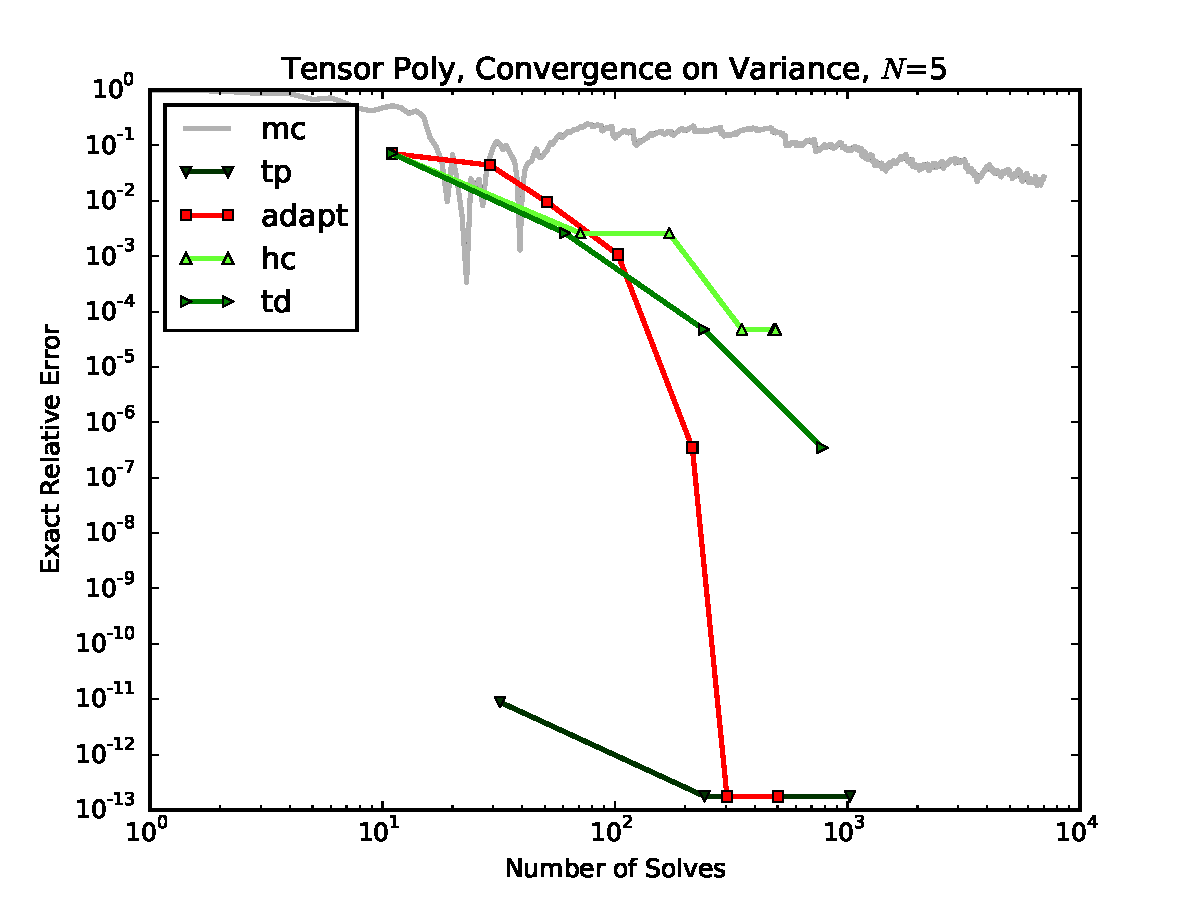
\includegraphics[width=0.7\linewidth]{tenspoly_varconv_5}
    \rule{35em}{0.5pt}
  \caption{Analytic $N=5$ Error Convergence, Variance}
  \label{fig:anl5_varconv}
\end{figure}
\begin{figure}[H]
  \centering
    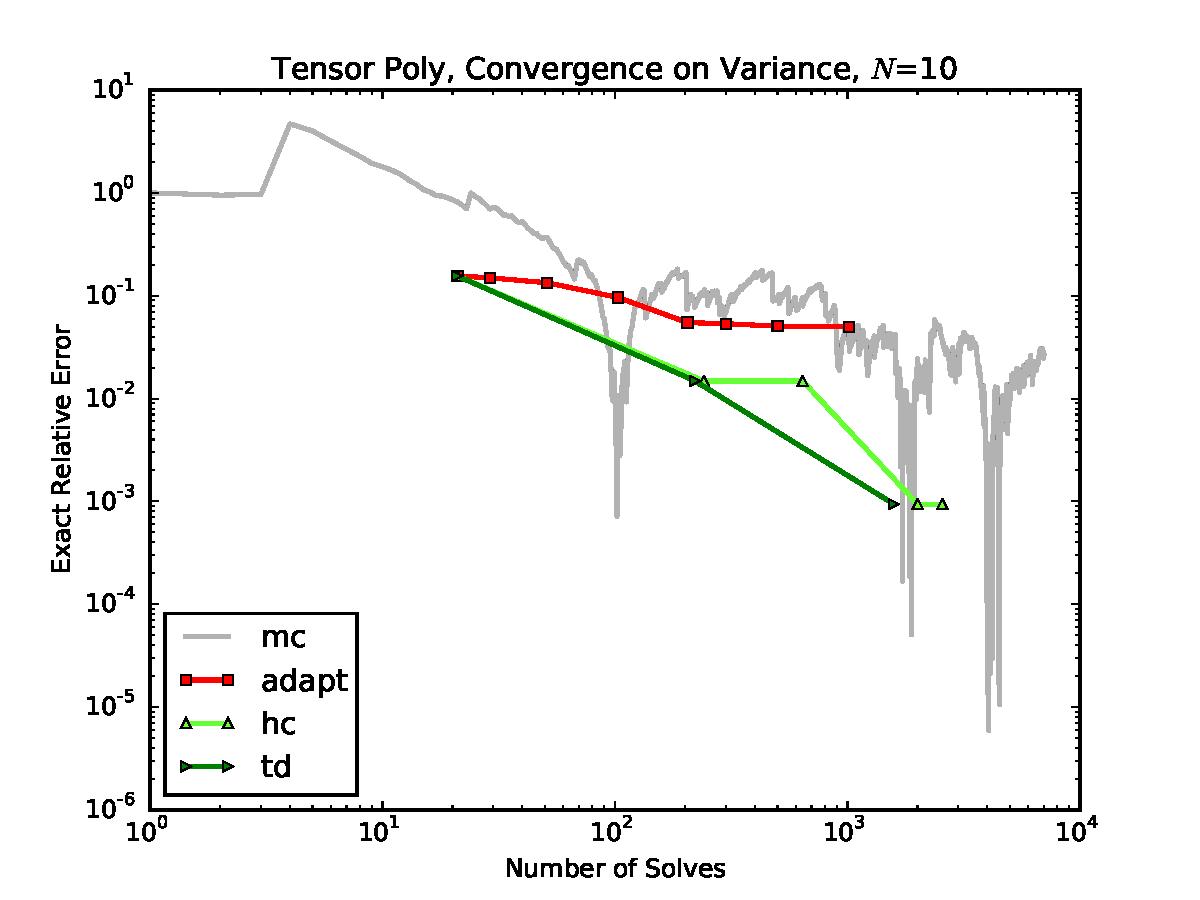
\includegraphics[width=0.7\linewidth]{tenspoly_varconv_10}
    \rule{35em}{0.5pt}
  \caption{Analytic $N=10$ Error Convergence, Variance}
  \label{fig:anl10_varconv}
\end{figure}



\section{Attenuation}
Similar to the polynomial model, the attenuation model does not converge exactly for any order of SCgPC
expansion, as exponential terms cannot be perfectly represented by a finite sum of polynomials.
Again distributing the input variables from 0 to 1, the mean and variance are
\begin{align}
  \text{mean}&=N^N\left(1-\exp(-\frac{1}{N})\right)^N,\\
  \text{var}&=\left(\frac{N}{2}\right)^N \left(1-\exp(-\frac{2}{N})\right)^N - \text{mean}^2,
\end{align}
where $N$ is the cardinality of the input space.  The convergence plots are shown in Figs.
\ref{fig:att5_varconv} and \ref{fig:att10_varconv}.

While considering this model, it is useful to expand the solution in a Taylor series for polynomial behavior.
In any one dimension,
\begin{equation}
  e^{-x} = 1 - x + \frac{x^2}{2!} - \frac{x^3}{3!} + \mathcal{O}(x^4).
\end{equation}
Because $y_n\in[0,1]$ and the nature of the polynomial expansion, we expect leading, low-order polynomial
terms to dominate the SCgPC expansion, and interactivity to be more dominant than high-order polynomials,
somewhat like the Polynomial Evaluations case above.

There are several notable features in this convergence graph that are not seen in the tensor polynomial case.
First, the Tensor Product and Total Degree index sets are very similar in exponential convergence; this is
somewhat expected given the polynomial expansions above.  Neither Total Degree nor Tensor Product ideally fit
this model as a low-order expansion, but both cover critical components of it as they grow in size.

The convergence of the Hyperbolic Cross index set is possibly the most striking result here.  The oscillatory
nature of the solutions covers a band wide enough to disguise any convergence after 100 computational solves.
It appears that the behavior is due to poor integration of high-order polynomial coefficients.  When a
polynomial is first added to the index set, insufficient quadrature is used to integrate the coefficient,
resulting in a large error for that coefficient.  However, when further points are added, the
poorly-integrated coefficient is resolved, and the variance converges more closely.  This behavior warrants
more investigation.

Lastly, we see some plateau behavior for the Adaptive SCgPC method. This is evidence of the adaptive algorithm
failing because of weaknesses in the search algorithm.



Interestingly, while the convergence of the adaptive method seems to be converging at a better rate than the
total degree isotropic set, there is no clear advantage for up to thousands of solves.  This is somewhat
expected, as there is coupling between inputs evident in the Taylor expansion of the attenuation model.  
As with the polynomial model,
the curse of dimensionality is clear.

\begin{figure}[H]
  \centering
    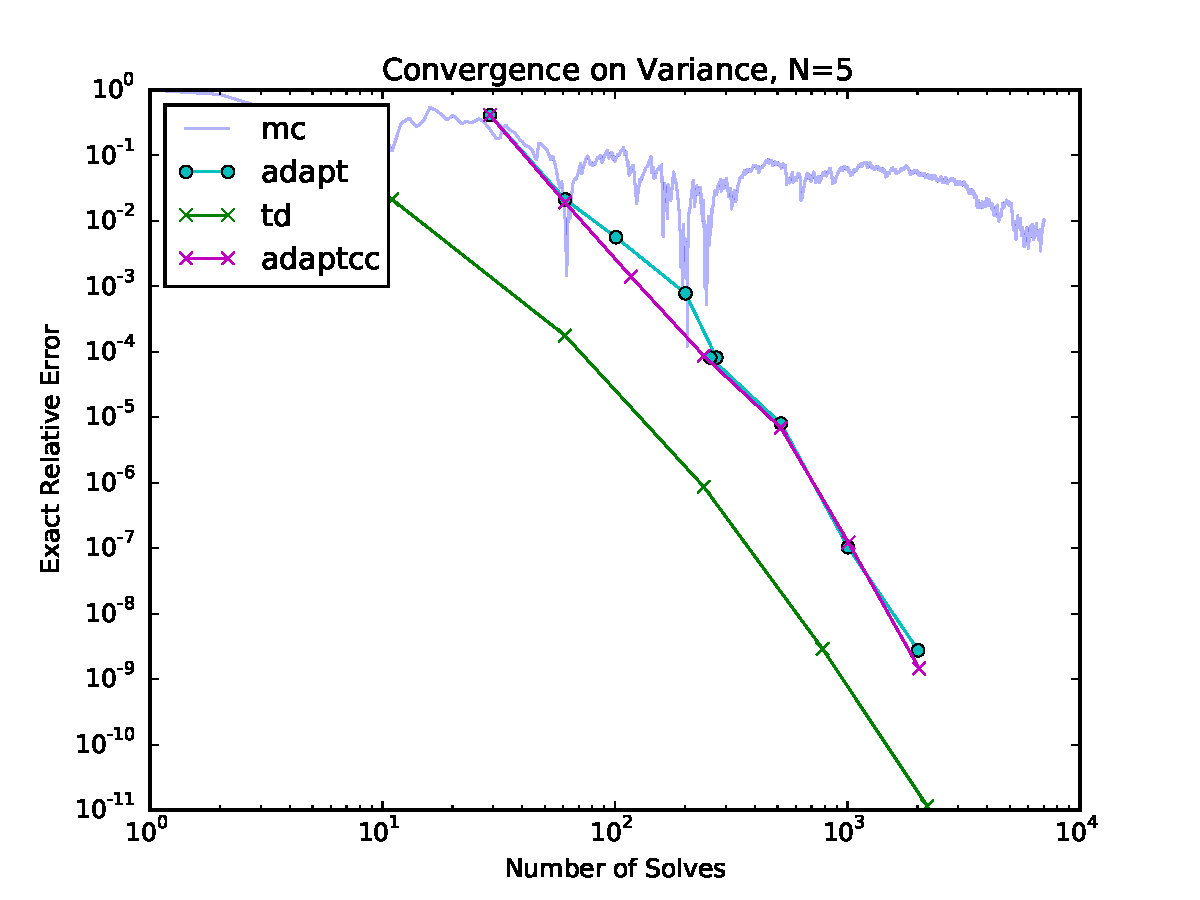
\includegraphics[width=0.7\linewidth]{attn_varconv_5}
    \rule{35em}{0.5pt}
  \caption{Attenuation $N=5$ Error Convergence, Variance}
  \label{fig:att5_varconv}
\end{figure}

\begin{figure}[H]
  \centering
    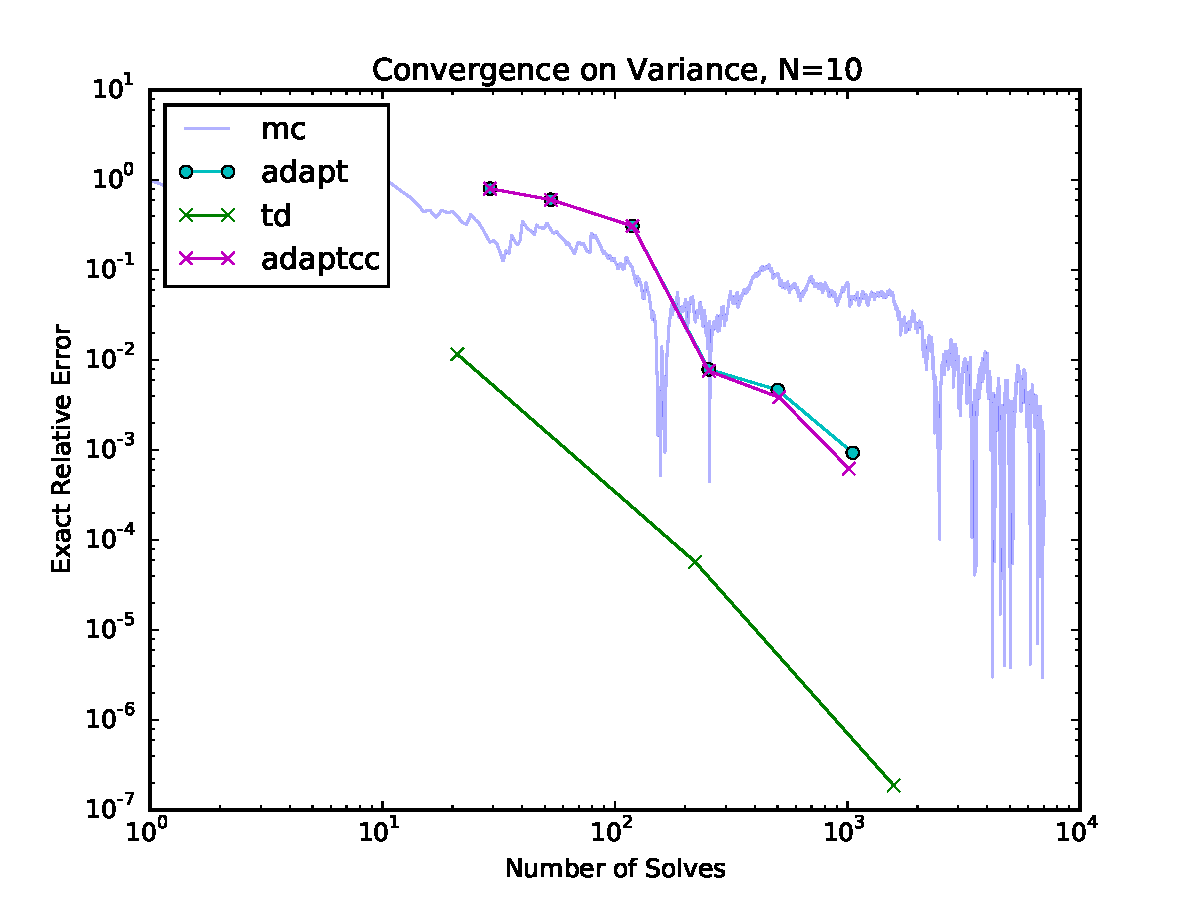
\includegraphics[width=0.7\linewidth]{attn_varconv_10}
    \rule{35em}{0.5pt}
  \caption{Attenuation $N=10$ Error Convergence, Variance}
  \label{fig:att10_varconv}
\end{figure}



%\section{Projectile}
%Unlike the attenuation and polynomial models, the projectile model is a nonlinear problem without an analytic
%solution.  As a result, the convergence benchmark is one achieved by a large Monte Carlo run, instead of an
%analytic benchmark; thus, the convergence of the various methods is limited to the convergence of the Monte
%Carlo point.  The most converged Monte Carlo point for this work is
%\begin{align}
%  \text{mean} = 1234, \\
%  \text{var} = 1234.
%\end{align}
%Additionally, this is the first model where significant anisotropy exists in the model.  For instance, the
%drag coefficient parameter is many orders of magnitude more influential on the quantity of interest than the
%gravitational acceleration.  
%The results in Fig. \ref{fig:proj_varconv} are interesting, and require additional data points to understand
%clearly.  However, we include Fig. \ref{fig:proj_varval} for clarity.  While it initially looks like the adaptive
%methods converge quickly, it appears that this is misleading, as shown in the values graph.  The adaptive
%method is converging, but passes through the benchmark value before turning back to converge on it.  This
%indicates the adaptive construction introduces too much variance initially, and additional terms are required
%to approach the benchmark solution.
%\begin{figure}[H]
%  \centering
%    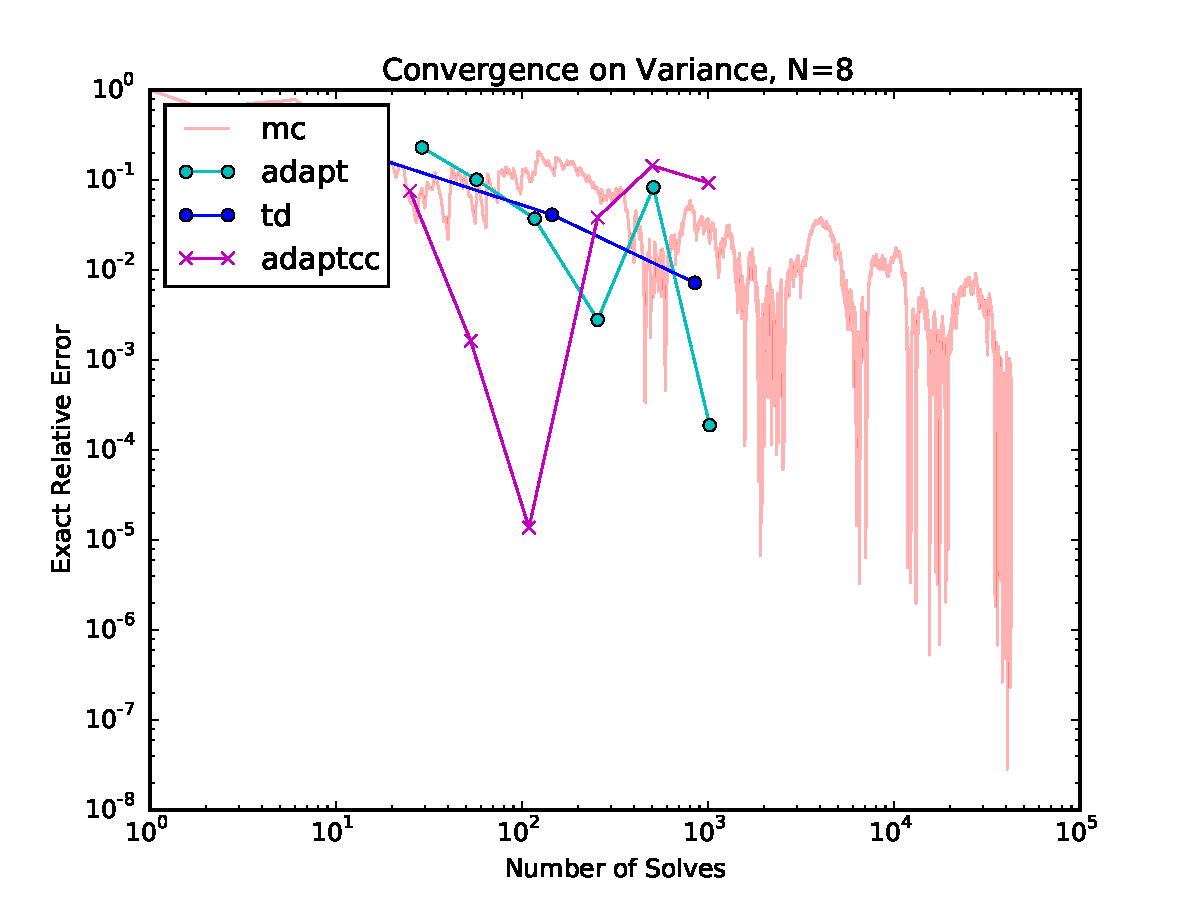
\includegraphics[width=0.7\linewidth]{proj_varconv_8}
%    \rule{35em}{0.5pt}
%  \caption{Projectile $N=8$ Error Convergence, Variance}
%  \label{fig:proj_varconv}
%\end{figure}
%\begin{figure}[H]
%  \centering
%    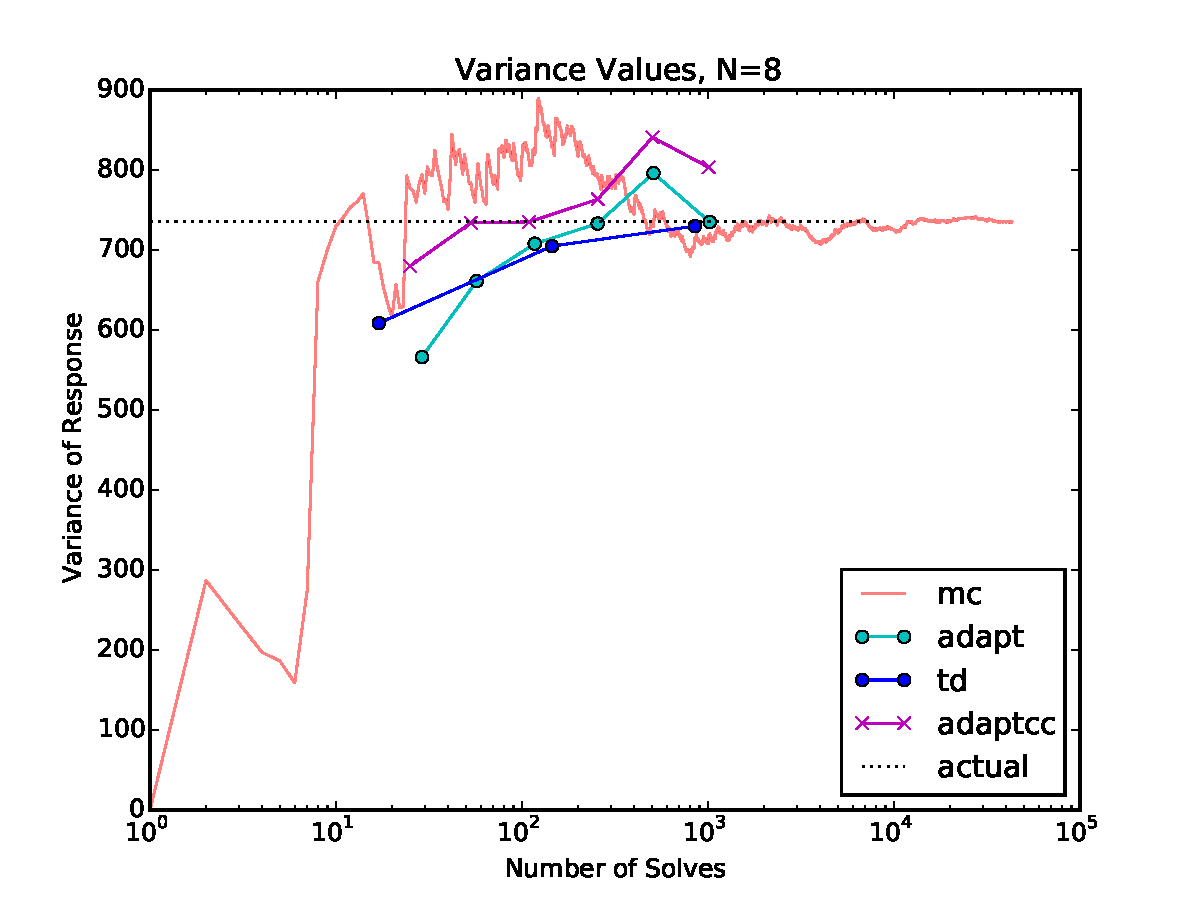
\includegraphics[width=0.7\linewidth]{proj_varvals_8}
%    \rule{35em}{0.5pt}
%  \caption{Projectile $N=8$ Values, Variance}
%  \label{fig:proj_varval}
%\end{figure}
%%\begin{figure}[H]
%% \centering
%%   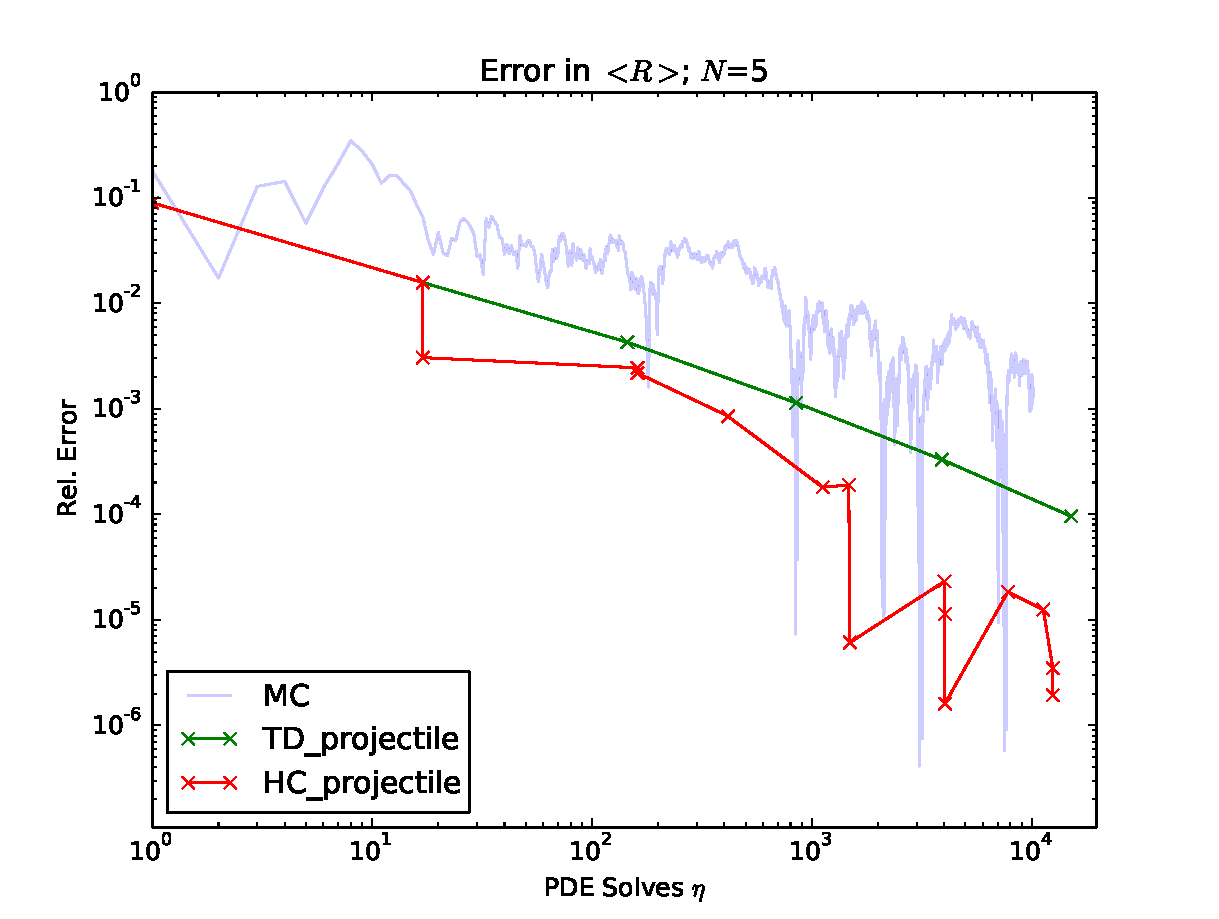
\includegraphics[width=0.7\linewidth]{projectile_errs}
%%    \rule{35em}{0.5pt}
%%  \caption{Projectile $N=8$ Error Convergence, Variance}
%%  \label{fig:proj_varconv}
%%\end{figure}
%


\section{Neutron Diffusion}
The neutron diffusion model is a complex, nonlinear model that begins to approach an engineering-scale model.
Because of complications with conflicting libraries, the adaptive SCgPC method was not available for this
model.  Particularly of note is the clear loss of convergence rate with increase in the
cardinality of the input space. %\{Note to self: fix coloring in plots.\}

\begin{figure}[H]
  \centering
    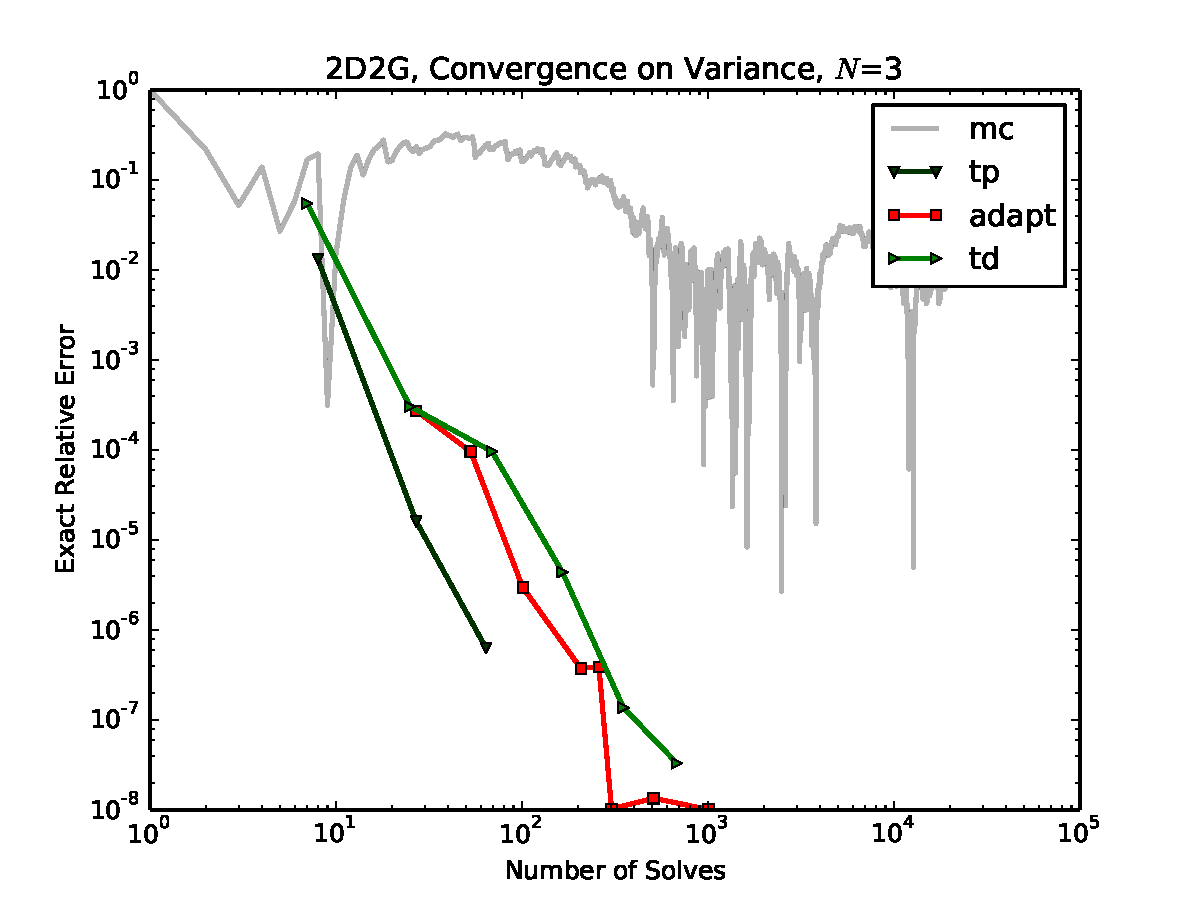
\includegraphics[width=0.7\linewidth]{2D2G_varconv_3}
    \rule{35em}{0.5pt}
  \caption{Diffusion $N=3$ Error Convergence, Variance}
  \label{fig:diff3_varconv}
\end{figure}
\begin{figure}[H]
  \centering
    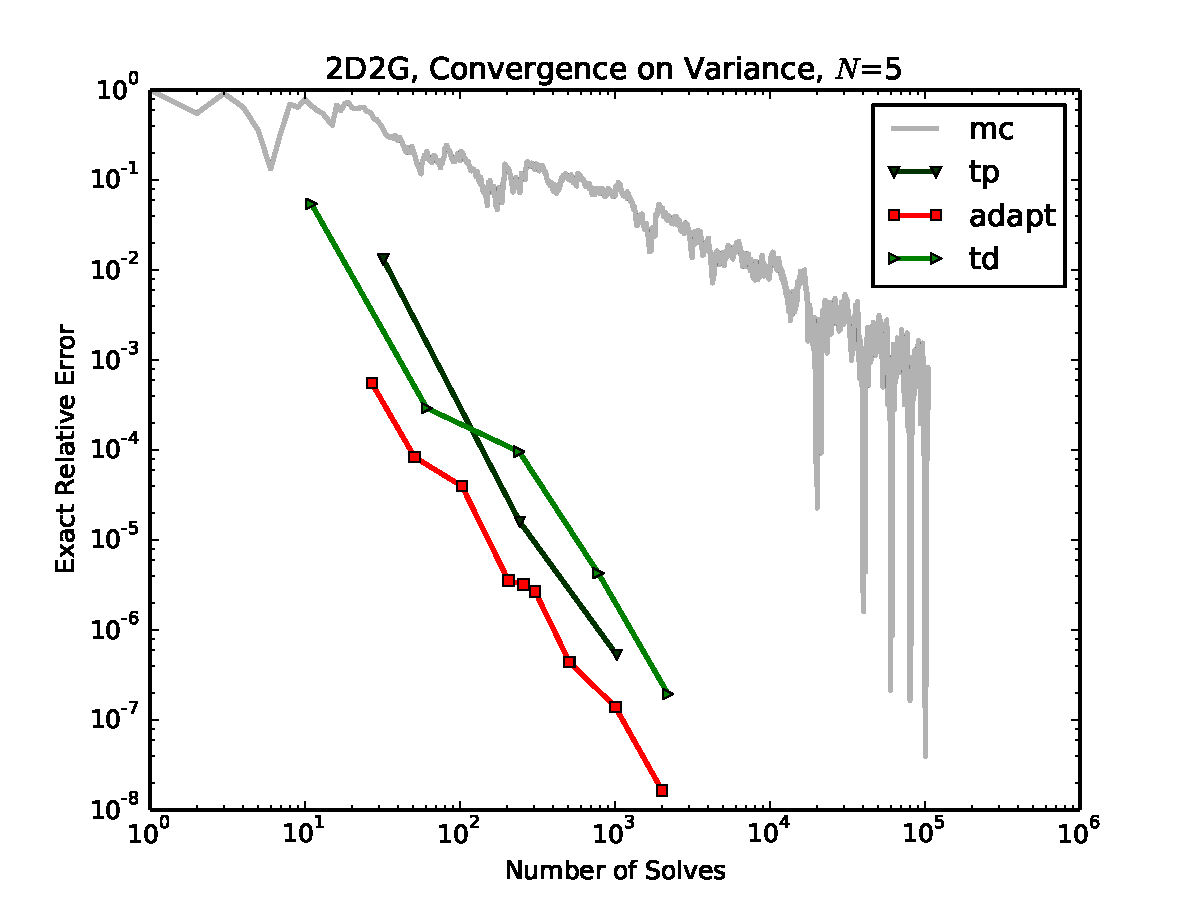
\includegraphics[width=0.7\linewidth]{2D2G_varconv_5}
    \rule{35em}{0.5pt}
  \caption{Diffusion $N=5$ Error Convergence, Variance}
  \label{fig:diff5_varconv}
\end{figure}
%\begin{figure}[H]
%  \centering
%    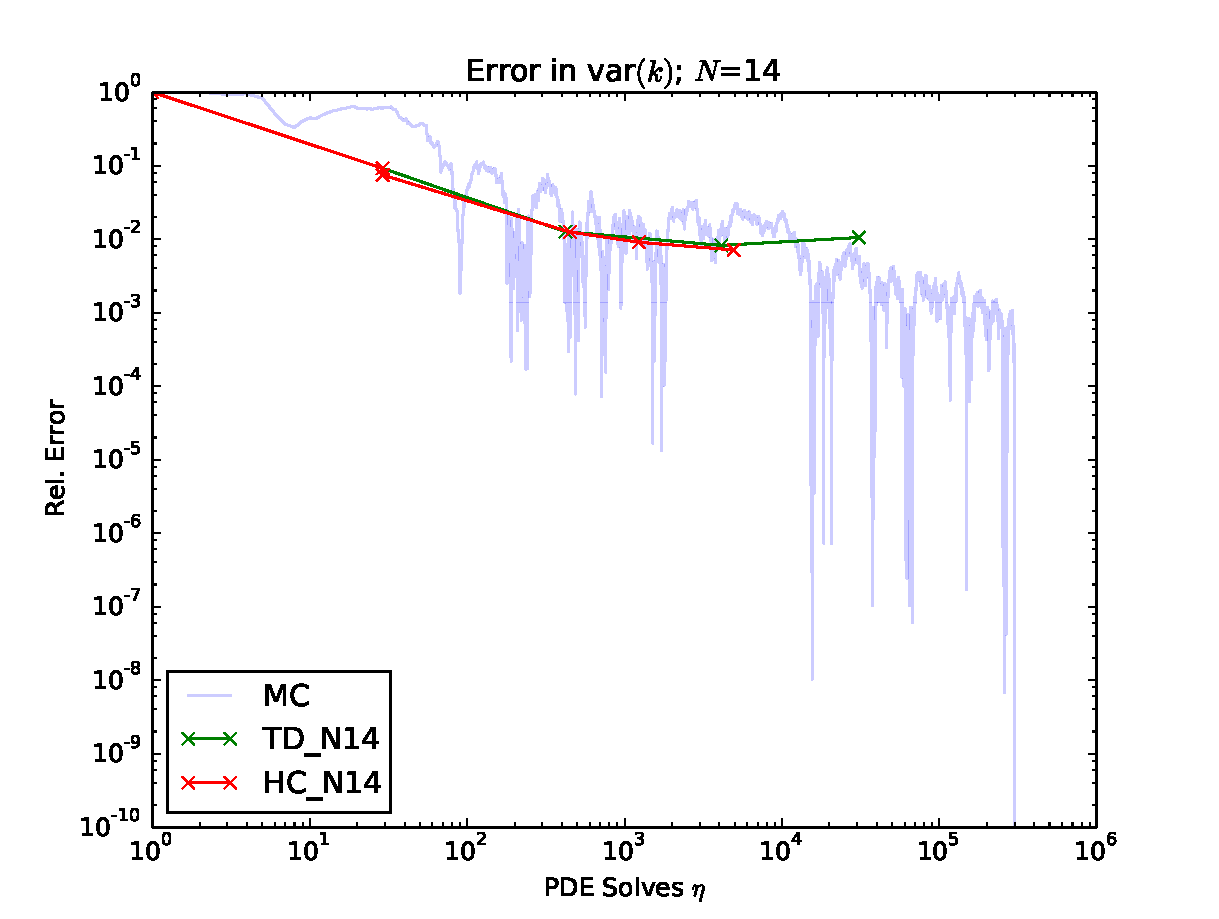
\includegraphics[width=0.7\linewidth]{N14_iso_var_errs}
%    \rule{35em}{0.5pt}
%  \caption{Diffusion $N=14$ Error Convergence, Variance}
%  \label{fig:diff14_varconv}
%\end{figure}





\section{Conclusions}
From evaluating the results using the various methods on these models, there are a few useful conclusions.

First, especially for models with small input cardinality, SCgPC methods tend to be faster converging than
traditional Monte Carlo methods.  In particular, the adaptive SCgPC method eventually exhibits exponential
convergence in the models considered here.  This is encouraging for many uncertainty quantification problems
where the variance is chiefly centered on a few input parameters.

%Second, using Clenshaw Curtis quadrature appears to have no negative consequence on converging with the
%adaptive SCgPC method, but no striking positive consequence either.  This suggests it is worth exploring other
%nested quadrature methods that might be beneficial in general, or at least in certain circumstances.

Second, it is clear that even with adaptive SCgPC, convergence is poor for input spaces with at least ten
inputs for less than a thousand solves.  For costly engineering codes, even a thousand runs may be
impractical, so further improvement of the adaptive algorithm is necessary.  This leads to the
proposed HDMR methods, which can further subdivide the input domain.  These subdivided domains have
cardinality much more suitable to SCgPC methods.

Lastly, because SCgPC methods improve drastically with decreases in input cardinality, we expect SCgPC to
benefit from coupling with input reduction methods, such as sensitivity-weighted input reduction through
principal component analysis using input-input covariance matrices.
